\documentclass[12pt,a4paper, reqno]{amsart}
% ukazi za delo s slovenscino -- izberi kodiranje, ki ti ustreza
\usepackage[slovene]{babel}
%\usepackage[cp1250]{inputenc}
%\usepackage[T1]{fontenc}
\usepackage[utf8]{inputenc}
\usepackage{amsmath,amssymb,amsfonts}
\usepackage{url}
%\usepackage[normalem]{ulem}
\usepackage[dvipsnames,usenames]{color}
\usepackage{graphicx}

% ne spreminjaj podatkov, ki vplivajo na obliko strani
\textwidth 15cm
\textheight 24cm
\oddsidemargin.5cm
\evensidemargin.5cm
\topmargin-5mm
\addtolength{\footskip}{10pt}
\pagestyle{plain}
\overfullrule=15pt % oznaci predlogo vrstico


% ukazi za matematicna okolja
\theoremstyle{definition} % tekst napisan pokoncno
\newtheorem{definicija}{Definicija}[section]
\newtheorem{primer}[definicija]{Primer}
\newtheorem{opomba}[definicija]{Opomba}

\renewcommand\endprimer{\hfill$\diamondsuit$}


\theoremstyle{plain} % tekst napisan posevno
\newtheorem{lema}[definicija]{Lema}
\newtheorem{izrek}[definicija]{Izrek}
\newtheorem{trditev}[definicija]{Trditev}
\newtheorem{posledica}[definicija]{Posledica}


% za stevilske mnozice uporabi naslednje simbole
\newcommand{\R}{\mathbb R}
\newcommand{\N}{\mathbb N}
\newcommand{\Z}{\mathbb Z}
\newcommand{\C}{\mathbb C}
\newcommand{\Q}{\mathbb Q}
\newcommand{\E}{\mathbb E}
\newcommand{\U}{\boldsymbol U}

% ukaz za slovarsko geslo
\newlength{\odstavek}
\setlength{\odstavek}{\parindent}
\newcommand{\geslo}[2]{\noindent\textbf{#1}\hspace*{3mm}\hangindent=\parindent\hangafter=1 #2}


% naslednje ukaze ustrezno popravi
\newcommand{\program}{Finančna matematika} % ime studijskega programa: Matematika/Finan"cna matematika
\newcommand{\imeavtorja}{Timotej Vesel} % ime avtorja
\newcommand{\imementorja}{prof.~dr./doc.~dr. Ime Priimek} % akademski naziv in ime mentorja
\newcommand{\naslovdela}{Mrežna pravila in kvazi-Monte Carlo metode za integracijo funkcij}
\newcommand{\letnica}{2019} %letnica diplome


% vstavi svoje definicije ...




\begin{document}

% od tod do povzetka ne spreminjaj nicesar
\thispagestyle{empty}
\noindent{\large
UNIVERZA V LJUBLJANI\\[1mm]
FAKULTETA ZA MATEMATIKO IN FIZIKO\\[5mm]
\program\ -- 1.~stopnja}
\vfill

\begin{center}{\large
\imeavtorja\\[2mm]
{\bf \naslovdela}\\[10mm]
Delo diplomskega seminarja\\[1cm]
Mentor: \imementorja}
\end{center}
\vfill

\noindent{\large
Ljubljana, \letnica}
\pagebreak

\thispagestyle{empty}
\tableofcontents
\pagebreak

\thispagestyle{empty}
\begin{center}
{\bf \naslovdela}\\[3mm]
{\sc Povzetek}
\end{center}
% tekst povzetka v slovenscini
V povzetku na kratko opi"si vsebinske rezultate dela. Sem ne sodi razlaga organizacije dela -- v katerem poglavju/razdelku je kaj, pa"c pa le opis vsebine.
\vfill
\begin{center}
{\bf Angle"ski naslov dela}\\[3mm] % prevod slovenskega naslova dela
{\sc Abstract}
\end{center}
% tekst povzetka v anglescini
Prevod zgornjega povzetka v angle"s"cino.

\vfill\noindent
{\bf Math. Subj. Class. (2010):} navedi vsaj eno klasifikacijsko oznako -- dostopne so na \url{www.ams.org/mathscinet/msc/msc2010.html}  \\[1mm]
{\bf Klju"cne besede:} navedi nekaj klju"cnih pojmov, ki nastopajo v delu  \\[1mm]
{\bf Keywords:} angle"ski prevod klju"cnih besed
\pagebreak



% tu se zacne besedilo seminarja
\section{Uvod}
\vspace{5mm }
\section{Neki}
\vspace{3mm }
Naš cilj je izračunati integral poljubne integrabilne funkcije $f$, ki je definiran na $s$-dimenzionalni hiperkocki $[0,1]^s$,
\[I(f) = \int_{0}^{1}\cdots \int_{0}^{1}f(x_1,\ldots,x_s)dx_1\cdots dx_s = \int_{[0,1]^s} f(\boldsymbol x) d \boldsymbol x.
\]
V praksi takšnega integrala za večino funkcij ne znamo izračunati eksaktno zato želimo izračunati numerični približek. Uporabili bi lahko kakšno deterministično (sestavljeno) integracijsko oziroma kvadraturno pravilo, npr. trapezno pravilo, Simpsonovo pravilo, 3/8 pravilo itd. To bi šlo, če bi bila dimenzija majhna (npr. $s = 4$), pri večjem številu integracijskih spremenljik pa se srečamo s t.i. \textit{prekletstvom dimenzionalnosti}.
Že pri $s = 40$ in samo dveh vozlih v vsaki smeri bi potrebovali $2^{40}$, kar je več kot bilijon izračunov vrednosti fukcije. (S poveprečnim računalnikom bi to trajalo ??? časa, zato za funkcije z veliko spremenljivkami potrebujemo druge metode.)

\vspace{5mm}
\section{Metoda Monte Carlo}
\vspace{3mm}
\textit{Metoda Monte Carlo (MC)} se uporablja za izračun približka pričakovane vrednosti $\E(X)$ slučajne spremenljvke $X$. Vzemimo  funkcijo $f : (0,1)^s \rightarrow \R$ in naj bo $ \boldsymbol{u} = (u_1,\ldots,u_s) \in (0,1)^s$ in $\boldsymbol{U} \sim \mathcal{U}(0,1)^s$ slučajni vektor (enakomerno porazdeljen na $s$-razsežni hiperkocki). Potem lahko zapišemo 
\[I(f) = \int_{0}^{1}\cdots \int_{0}^{1}f(u_1,\ldots,u_s)du_1\cdots du_s = \int_{[0,1]^s} f(\boldsymbol u) d \boldsymbol u = \E[f(\boldsymbol U]
\]
\begin{izrek}[Krepki zakon velikih števil Kolmogorova]
Naj bodo $X_1,X_2,\ldots,X_n$ neodvisne in enako porazdeljene slučajne spremenljivke na skupnem verjetnostnem prostoru, za katerega obstaja pričakovana vrednost $\E(X_i) = \mu$. Tedaj zaporedje vzorčnih povrpečij $S_n = \frac{X_1 + \ldots + X_n}{n}$ skoraj gotovo konvergira k $\mu$.
\end{izrek}
KZVŠ nam torej zagotavlja, da bo za večji $n$ $S_n$ boljši približek za matematično upanje in posledično je 
\[
\E[f(\U] \approx \frac{f(\U_1) + \ldots+ f(\U_n)}{n}
\]
\vspace{2mm}

Klasična Monte Carlo Metodo zato $\E[f(\U)$ oziroma $I(f)$ aproksimira z 
\[Q_n(f) = \frac{1}{n} \sum_{i=0}^{n-1} f(\U_i)
\]
kjer so $\U_0,\ldots,\U_{n-1}$ neodvisni $\mathcal{U}(0,1)^s$ slučajni vektorji.  V implementaciji slučajne vektorje $\U_i$ zamenjamo z vektorji ``(psevdo) naključnih števil''.
To je zelo preprosta ter široko uporabljena metoda.

Poleg tega opazimo, da je $Q_n(f)$  nepristranska cenilka za $\E[f(\U)] = I(f)$, t.j. $\E[Q_n(f)] = \E[f(\U)]$:
\[
\E[Q_n(f)] = \E\left( \frac{1}{n} \sum_{i=0}^{n-1} f(\U_i)\right) = \frac{1}{n}  \sum_{i=0}^{n-1}\E[ f(\U_i)] =\E[f(\U)].
\]
\vspace{2mm}

Izračunamo lahko še srednjo kvadratično napako, ki nam pove koliko se približek integrala (cenilka) razlikuje od točne vrednosti integrala:
\vspace{2mm}
\[
\begin{split}
SKN[Q_n(f)] & = \E[(Q_n(f) - \E[f(\U)] \\
& = \E[(Q_n(f) - \E[Qn(f)]] = \\
& = Var[Q_n(f)] \\
& = Var\left(\frac{1}{n} \sum_{i=0}^{n-1} f(\U_i)\right) \\
& = \frac{1}{n^2}  \sum_{i=0}^{n-1} Var[f(\U_i)]\\
& = \frac{Var[f(\U)]}{n},
\end{split}
\]
kjer je $\sigma^2_f = Var[f(\U)] = \int_{(0,1)^s} f^2(\boldsymbol u) d \boldsymbol u - I^{2}(f)$ in zadnja enakost velja, ker so $\U_i$ neodvisni in enako porazdeljeni slučajni vektorji.
Parameter  $\sigma^2_f$ nam ponavadi ni eksplicitno poznan, vendar ga lahko statistično ocenimo z vzorčno disperzijo 
\[
S^2 = \frac{1}{n-1}\sum_{i=0}^{n-1}(f(\U_i) - Q_n(f))^2.
\]
Iz tega sledi, da je koren iz srednje kvadratične napake enak $S/\sqrt{n}$.
Pravimo, da je konvergenca Monte Carlo Metode reda ``$1/\sqrt{n}$'', kar označimo z $\mathcal {O}(1/\sqrt{n})$.Red konvergence je neodvisen od dimenzije problema. Takšen red konvergence v praksi pomeni, da če bi želeli napako prepoloviti, bi za to potrebovali štirikrat več vzorčnih točk (slučajnih spremenljivk).

Izkaže se, da so za probleme nizkih dimenzij determistična integralska pravila učinkovitejša za gladke funkcije, v višjih dimenzijah pa so Monte Carlo metode veliko hitrejše.

Kljub temu, da so Monte Carlo metode večinoma hitrješe od kvadaturnih pravil in so zelo široko uporabljene, pa je red konvergence  $\mathcal {O}(1/\sqrt{n})$ velikokrat prepočasen za praktično uporabo. Za zmanjšanje variance obstajajo različne tehnike (npr. stratifikacija), vendar v praksi MC metode pogosto ostanejo prepočasne.

\vspace{5mm}
\section{Kvazi-Monte Carlo metode}
\vspace{3mm}

\textit{Kvazi-Monte Carlo (QMC) metode} so deterministična različica Monte Carlo metod. Pri QMC metodah zamenjamo neodvisne slučajne točke $\U_i$ z množico determinističnih  točk, ki hiperkocko $[0,1)^s$ pokrijejo bolj enakomerno.

 Recimo, da je naš cilj izračunati:
\[
I(f) = \int_{[0,1)^s} f(\boldsymbol u)d\boldsymbol u.
\] 
Opazimo, da je območje integracije nekoliko drugačno kot pri MC metodi, kjer je vseeno ali vključimo robove hiperkocke. Pri QMC pa so nekater metode takšne, da imajo deterministične točke pogosto koordinate v 0, prav tako to zahtevajo nekatere definicije, ki jh bomo potrebovali za QMC .

QMC ocena zgornjega problema pa je podobna oceni za standardno MC metodo.

\begin{definicija}{(Kvazi-Monte Carlo ocena).} 
Naj bodo $\boldsymbol u_0,\boldsymbol u_1,\ldots,\boldsymbol u_{n-1}$ (``deterministično'') izbrane točke v hiperkocki $[0,1)^s$. QMC ocena integrala $I(f)$ je definirana kot
\[
\overline{I}_{QMC} = \frac{1}{n} \sum_{i=0}^{n} f(\boldsymbol u_i).
\]
\end{definicija}
\vspace{1mm}

\begin{definicija}{(Diskrepanca??)}.
Naj bo $\mathcal{B}$ družina vseh podmnožic $B \subset[0,1)^s$. Diskrepanca množice točk $P = \{\boldsymbol x_1,\ldots,\boldsymbol x_n\}$ je definirana kot

\begin{equation}
D_n(P) =\sup\limits_{B \in \mathcal{B}}\left\lvert\frac{\sum_{i = 1}^n \mathbb {I}_B(\boldsymbol x_i)}{n} - \lambda(B) \right\rvert,
\end{equation}
kjer je 
\vspace{2mm}
\[
\mathbb{I}_B(\boldsymbol x_i) =
  \begin{cases}
  1; & \mbox{točka $\boldsymbol x_i$ je v množici $B$,} \\	
  0; & \mbox{sicer}$$
  \end{cases}
  \] 
  \\[2mm]
 in $\lambda(B)$ je Lebesgueova mera?? oziroma, ker je $B$ $n$-dimenzionalna škatla ( n-orthotope??), kar $n$-dimenzionalni volumen???) množice $B$.
\end{definicija}


\begin{definicija}{(Star Discrepancy)}. Naj bo $\mathcal{J}^*$ družina vseh podinteravalov $J^*\subset [0,1)^s$ oblike $\prod\limits_{i=1}^s [0,u_i), 0 \leq u_i \leq 1$ (poznani tudi kot ??zasidrane škatle?? anchored boxes), the star discrepancy?? množice točk $P=\{\boldsymbol x_1, \ldots, \boldsymbol x_n \}$ v $[0,1)^s, D^*_n(P)$, je definirana kot v enačbi (1) z $\mathcal{J}^* = \mathcal{B}$.
\end{definicija}

Slika 1 prikazuje to diskrepanco. Na sliki so zasidrana škatla $[0,a) = [0,0.4) \times [0,0.8) \in [0,1)^2$ in množica $n=20$ točk. Zasidrana škatla vsebuje 5 izmed 20 točk, zato je $\frac{1}{n}\sum_{i = 1}^n \mathbb {I}_{0\leq \boldsymbol{x}_i<a} (\boldsymbol x_i)=0.20$. Ploščina (volumen) zasidrane škatle pa je 0.32, zato je $|0.2 - 0.32|=0.12$. The star diskrepanco $D_{20}^*$ najdemo z maksimiziranjem razlike po vseh zasidranih škatlah $[0,a)$.

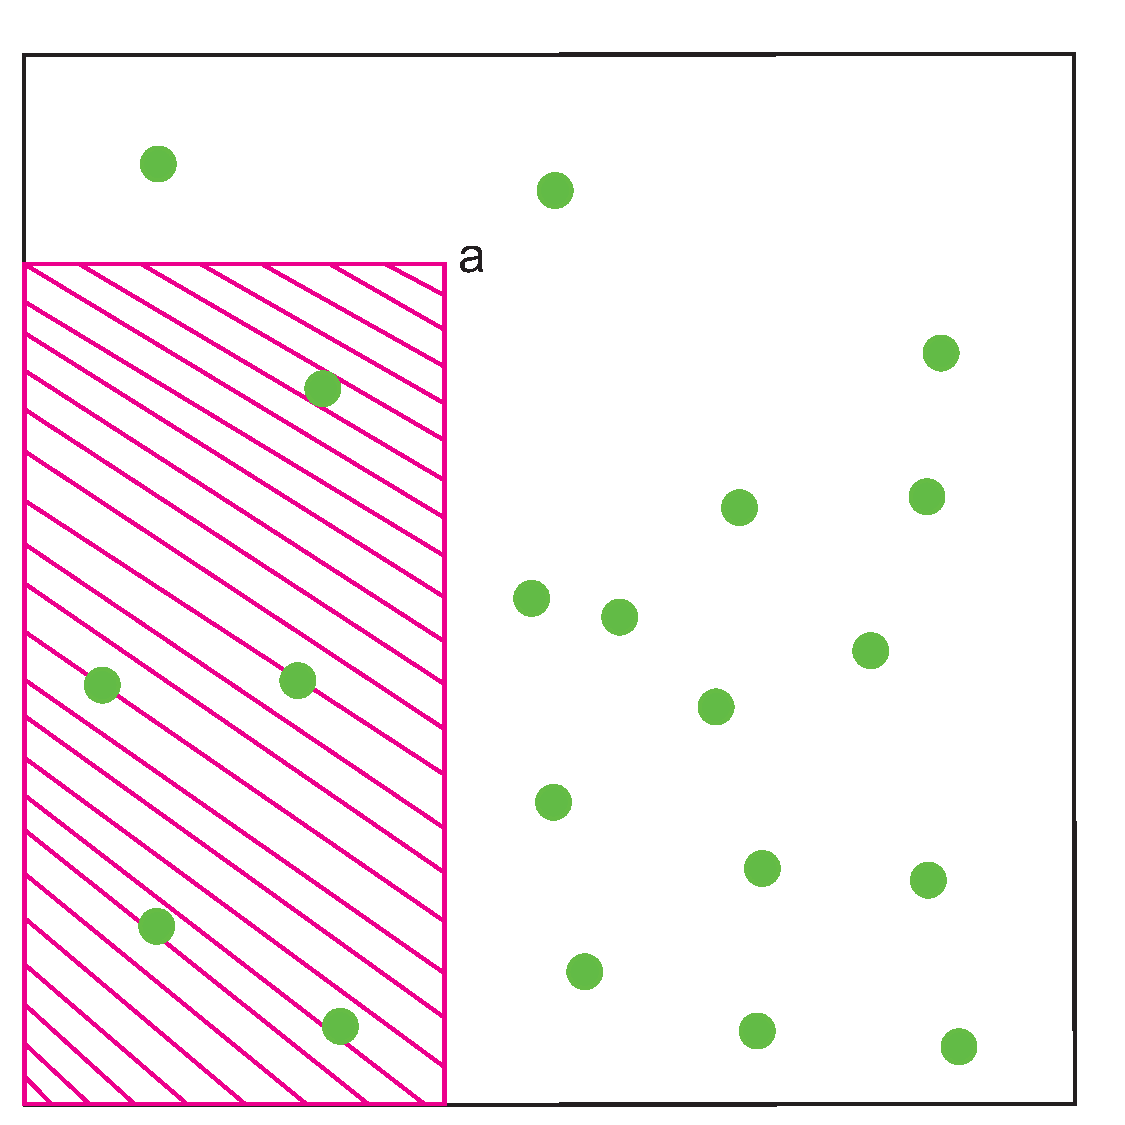
\includegraphics [width=14cm, height=14cm]{discrepancy.pdf}
\vspace{3mm}

\noindent Slika 1: V enotskem kvadratu je prikazanih 20 točk in zasidrana škatla (senčeno) od $(0,0)$ do $a = (0.4,0.8)$. zasidrana škatla ima ploščino 0.32 in vsebuje $5/20 = 0.2$ vseh točk. 

\vspace{3mm}
Za $\boldsymbol{x}_i \sim \mathcal{U}[0,1)^s$ je Chung pokazal, da je
\begin{equation}
\limsup_{n \to \infty} \frac{\sqrt{2n}D_n^*}{\sqrt{log (log(n))}} = 1,
\end{equation}
torej je $D_n^* = \mathcal{O}((\frac{log\mbox{ }log(n)}{n})^\frac{1}{2})$ z verjetnostjo 1. Ko se $n$ povečuje, logaritem raste zelo počasi, zato bo $D_n^*$ le malo boljša kot $\mathcal O(1/\sqrt{n})$ za velike $n$.
\vspace{3mm}

Znano je, da lahko z deterministično izbiro točk $\{\boldsymbol{x}_i \}$ dosežemo, da je $D_n^*$ veliko manjši kot (2).
Obstajajo neskončna zaporedja  $\{\boldsymbol{x}_i \}$ v $[0,1)^s$ z $D_n^*(\boldsymbol x_1,\ldots, \boldsymbol x_n) = \mathcal O(log(n)^s/n)$. Takšna zaporedja se imenujejo \textit{zaporedja z nizko diskrepanco?? (low-discepancy sequences)} in njih na temeljijo Kvazi-Monte Carlo metode.

\begin{definicija}{(Zaporedja z nizko diskrepanco)}.
Zaporedje točk $P = \{\boldsymbol x_n\}_{n\in \N} \subset [0,1)^s$ se imenuje zaporedje z nizko diskrepanco, če je star discerpancy  $D^*_n(P)$ prvih $n$ točk množice $P$ enaka $\mathcal{O}(\frac{log (n)^s}{n})$.
\end{definicija}

Obstaja povezava med manjšo diskrepanco in bolšjim približkom za integral. Povezuje jo \textit{Hlawka-Koksma neenakost?}.
\vspace{2mm}
\begin{izrek}[Neenakost Hlawka-Koksma]
Naj ima funkcija f variacijo? V(f) v smislu Hardy-Krause. Potem za poljubno množico točk $P = \{\boldsymbol{x}_1,\ldots,\boldsymbol{x}_n\}$ v $[0,1)^s$ velja

\begin{equation}
\left\lvert\frac{\sum_{i=1}^{n} f(\boldsymbol{x}_i}{n} - \int_{[0,1)^s} f(\boldsymbol{x})d\boldsymbol{x} \right\rvert \leq V(f)D_n^*(P).
\end{equation}
\end{izrek}
\vspace{4mm}

Definicija za V(f)??? (podana je v [26] Harald Niederreiter. Random Number Generation and Quasi-Monte Carlo
Methods. S.I.A.M., Philadelphia, PA, 1992.)


% slovar
%\section*{Slovar strokovnih izrazov}

%\geslo{}{}
%
%\geslo{}{}
%


% seznam uporabljene literature
%\begin{thebibliography}{99}

%\bibitem{}

%\end{thebibliography}

\end{document}

